%%==================================================
%% chapter01.tex for BIT Master Thesis
%% modified by yang yating
%% version: 0.1
%% last update: Dec 25th, 2016
%%==================================================
\chapter{绪论}
\label{chap:intro}
\section{研究背景}

随着互联网的迅猛发展,各种应用软件日益增多,软件规模越来越大,但是这些软件背后的软件安全及其稳定性的问题也日益突出。尤其是在越来越多的无人场景下,如无人驾驶领域,软件正逐步完全代替人类的角色,这就对软件的安全性[1]提出了更高的要求。

任何的软件设计或者编码带来的安全隐患漏洞[2],都可能成为潜在的安全隐患,可能会给社会带来巨大的损失,信息安全问题早就成为人们日益关注的焦点[3]。近年来,重大网络安全事件层出不穷,如2017年5月,史上规模最大的一次勒索病毒攻击事件爆发,全球近百个国家的网络遭遇Wannacry病毒[4]的攻击,电脑被该病毒感染后文件会被加密锁定,支付黑客索要的赎金后才能解密恢复,受攻击对象甚至包括医院、高校等公益性机构。2013年6月,前美国中情局(CIA)雇员斯诺登曝出一项由美国国家安全局(NSA)实现的棱镜计划[5],震惊全球。据斯诺登披露的资料显示,NSA通过植入恶意软件感染了全球超过5万台计算机,用于窃取敏感信息;

由于软件的复杂性随着软件的规模和数量不断增大,软件开发的规模和数量不断增大,软件开发的难度也在增大,导致在开发过程中存在某些不确定性的错误或缺陷。另一方面软件开发人员的水平参差不齐,即使是富有经验的开发者在开发过程中也难以避免引入一些错误或缺陷。如图1所示,Eclipse3.0.1中也会存在着一些明显的空指针引用错误[6]。公开数据显示,对于有经验的程序员编写的代码,每1000行就有50-250个错误,平均每1000行会有100个缺陷,即使是经过软件故障控制管理培训的软件工程师,平均每1000行代码中存在50个故障[7]。因此,整个行业在关注软件如何提升生产力的同时,也更加注重提高软件源代码编写的质量,加大了对源代码的检测力度,以期及早发现代码中潜在的安全隐患,避免或减少因为软件缺陷带来的损害。据统计,现在在软件开发总成本中,投入到软件测试中的资源约占到25%到50%[8],并贯穿到软件生命周期的各个阶段。

 \begin{figure}
 \centering
 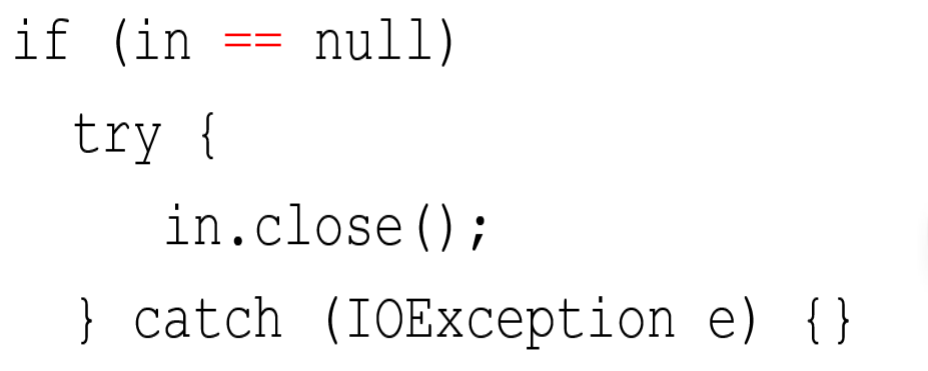
\includegraphics[width=0.50\textwidth]{figures/NullPointer1-1}
 \caption{Eclipse3.0.1中存在的空指针引用缺陷}\label{fig:diagram}
\end{figure}

目前的软件缺陷检测技术主要分为两种:静态检测和动态检测。 

动态检测[9]主要侧重于软件的性能、功能完善等方面,通过动态测试来进行漏洞的探测与发现,不仅仅要求测试人员对缺陷特性具有较深入的理解,测试过程中还需要大量测试用例,在目前软件规模愈加庞大,逻辑愈加复杂的情境下,这种方式必然带来大量的人力和物力的浪费。静态检测[10]是指利用静态分析手段来探测程序中潜在缺陷的方法,不需要运行程序使用其他手段完成对程序结构分析的技术。相较于动态分析技术而言,静态分析成本较低,而且能有效的对代码中的缺陷进行精确定位。因此,对源代码的静态分析和缺陷检测是一个值得深入研究的方向。

\section{国内外研究现状及发展趋势}
%\label{sec:***} 可标注label
通过人们对故障的总结,人们发现常见的比较大型的软件故障有数组越界,资源泄漏,空指针引用等,其中空指针引用问题出现的尤为频繁,根据coverity公司2009年针对280个开源项目的故障分析报告,空指针引用在所有类故障中所占比例为27.81%,是所占比例最高的故障[11]。

Null关键字的广泛使用是Java代码中产生NPE(Null Pointer Exception)故障的直接原因,Haidar Osman[12]等人开发了NullTracker工具对810个开源Java项目进行简单的数据流分析,追踪代码中空指针检查语句的分布情况,以发现程序开发者使用null关键字的时机和目的,结果表明在所有的条件判断语句中,用来进行空指针检查的语句平均占比为35%,类成员没有初始化,方法返回null值,以及向方法中传递null值是引发NPE的最常见的因素。其中,71%的空指针检查语句用来保证方法调用返回值的安全性。由于空指针检查语句的频繁使用,可能导致程序运行时的开销增加2%-10%,不仅如此,空指针检查的频繁使用还会降低代码的可读性和可维护性,而一旦缺失了这种检查,程序的稳定性便无法得到保障。

现在已有一些检测空指针引用的工具和技术,相关技术可粗略的分为指针引用验证和空指针引用[13]缺陷检测两大类;前者侧重于如何验证程序中的指针是否为空。后者侧重于如何尽可能多的发现程序中的空指针引用。指针引用验证技术是基于需求驱动的思想[14],一般是首先识别出指针,再沿着控制流后向的验证指针是否为空。空指针引用缺陷检测一般是在进行数据流分析[15]、指针分析的基础上,根据一些规则基于控制流前向的检测。两者通常都需要进行数据流分析与指针分析。

Salsa[16]是一个致力于验证Java代码中指针引用安全性验证的工具,通过定制的数据表示形式进行前向数据流分析,通过对传播深度和数据流传播路径数量的简单限制来获得方法的可扩展性,同时依赖预先进行的必然别名分析来提高方法间数据流分析的准确性。由于一些空指针的引用需要经过多层方法调用链才有可能触发,这种验证方式会产生一些漏报。

Ravichandhran Madhavan[17]等提出了一种过近似的最弱前置条件分析方法以验证Java程序中指针的安全性,该方法通过需求驱动的前向数据流分析,试图找到程序入口处可能满足被分析程序点的引用不安全的条件,如果存在这样的条件,则可以判定该引用不安全。此方法的数据流事实为有限的谓词集合,通过有选择地限制谓词集合的大小以及传播路径的数量,该方法可以做到低延迟的流敏感,上下文敏感的sound分析,利用Wala[18]程序分析框架,可以取得较好的验证引用安全的效果,但是过于追求针对单个引用的需求驱动分析,在对大规模代码中的引用进行批量分析时性能欠佳。

在工业界,空指针检测相相比于指针安全性验证更加具有实用性,而误报率和漏报率是检验工具实用性的重要指标,空指针检测工具大多不追求完美的正确率,而将较低的误报率和较高的召回率作为最重要的目标。

FindBugs[6][19]是一个开源的针对Java代码的缺陷静态检测工具,通过分析class文件,在字节码层级进行简单的前向数据流分析,对程序中的每一个引用的是否为null值的不同情况,给定相应的标识从而在触发可能的空指针调用时给出不同的告警等级。对于指针引用FindBugs总结出了一些经验规则,对不可达路径、控制流汇合、指针赋值语句、断言等特定情况定制了专用的检测规则,在进行过程间分析时,其主要依赖特定故障模式以及用户编码时给出的注解来推断空指针是否可能发生,所以它只能检测出特定场景下的空指针引用。

检测工具Xylem[20]从每一个指针引用出发,进行基于需求驱动的后向数据流分析,并将谓词作为数据流事实,目标是能够高效的检测出最重要的空指针引用,在进行分析时采取的是不完全可靠的分析方法,检测结果存在较多漏报。

杨睿[21]提出一种Java中空指针引用故障的静态检测方法,将空指针引用问题抽象为一类故障模型,并以故障模式状态机来形式化描述此类故障模型,然后根据故障状态机的创建条件及待检测代码的语义信息确定是否创建该类型的状态机,并将创建的状态机示例置于控制流图入口,根据数据流分析的结果对故障状态进行迭代以检测空指针引用问题。

姜淑娟[22]提出一种空指针异常自动定位方法,该方法结合程序的静态分析技术,利用程序运行时的堆栈信息指导程序切片,然后对得到的切片进行空指针分析及别名分析,得出引发空指针异常的可疑语句集合,最终给出错误定位报告。

以上这些分析方法都有各自的优缺点,目前无法找到一种完美的方法兼顾缺陷检测的误报率和漏报率,因此本课题提出使用多种工具交叉检测缺陷的方法,在降低漏报率的同时,通过对缺陷可信度的排序在某种程度上也降低了检测的误报率。

\section{本文研究内容}
%\label{sec:***} 可标注label
1. 交叉验证现有的空指针引用缺陷静态检测工具

静态分析技术与工具具有较早发现缺陷、覆盖率高、低开销、自动化程序高等优点;同时静态分析技术也存在一定的局限性,不仅要在分析效率与精度中做出取舍,还需要在误报率与漏报率之间做出取舍。现有的一些静态检测工具(如Findbugs,PMD)都采用了不同的实现方法达到这样的平衡,由于采取的分析策略的不同,形成的检测结果也往往有较大差异。

在本课题研究的第一阶段,我们主要通过构造的测试用例以及部分开源工程交叉验证现有的一些静态代码检测工具,考察其对不同类型空指针引用缺陷的检测能力(检测结果的准确率),同时对空指针引用缺陷类型进行分类,进而确定空指针缺陷检测的重点和难点,为下一步的研究工作进行铺垫。

2. 实现空指针引用缺陷的静态检测工具

在本课题研究的第二阶段,通过分析第一阶段获取的数据,重点研究现有工具不能覆盖的空指针引用缺陷类型,利用数据流分析技术实现空指针缺陷检测工具。

数据流分析是静态分析技术中的一种,是在不运行程序的前提下,静态计算出程序运行时变量和表达式的值。数据流分析是对程序进行近似计算,通常是计算出每个程序点上所分析对象的所有可能取值的集合。程序点上各分析对象的取值数据流值通常称为数据流事实,一个程序点处的状态为程序运行时刻到该点时的所有变量的值。

本阶段的工作主要利用现有的静态分析工具构建Java程序的控制流图和方法调用关系图,然后利用数据流分析技术建立分析模型,最终完成空指针引用缺陷检测工具,与现有工具形成互补关系。具体工作有以下几点:

(1)构建方法内的控制流图以及方法间的方法调用图;

(2)抽象合理的数据流事实模型,确定分析模式,同时建立数据流流经不同节点时的转换函数;

(3)针对过程间分析时的数据流传输设计合理方案;

(4)针对特殊数据结构,库方法调用等特殊问题设计解决方案;

(5)利用第一阶段使用的测试数据集验证检测能力;

3. 将工具集成至SonarQube平台

SonarQube是一个用于代码质量管理的开源平台,通过插件机制,Sonar 可以集成不同的测试工具,代码分析工具,以及持续集成工具,比如pmd-cpd、checkstyle、findbugs、Jenkins。通过不同的插件对这些结果进行再加工处理,通过量化的方式度量代码质量的变化,从而可以方便地对不同规模和种类的工程进行代码质量管理。

本阶段将把现有的静态分析工具及第二阶段实现的工具以插件的形式集成至SonarQube平台。在检测Java代码的过程中,比对不同检测工具生成的检测报告,根据各个工具对于不同类型空指针引用缺陷的检测能力对检测结果进行可信度排序,最终把检测出的空指针引用缺陷以可信度优先级排序的形式展示。




\subsection{形状记忆聚氨酯的形状记忆机理}
%\label{sec:features}

形状记忆聚合物(SMP)是继形状记忆合金后在80年代发展起来的一种新型形状记忆材料\upcite{Jiang2005Size}。形状记忆高分子材料在常温范围内具有塑料的性质,即刚性、形状稳定恢复性;同时在一定温度下(所谓记忆温度下)具有橡胶的特性,主要表现为材料的可变形性和形变恢复性。即“记忆初始态-固定变形-恢复起始态”的循环。

固定相只有物理交联结构的聚氨酯称为热塑性SMPU,而有化学交联结构称为热固性SMPU。热塑性和热固性形状记忆聚氨酯的形状记忆原理示意图如图\ref{fig:diagram}所示

\begin{figure}
 \centering
 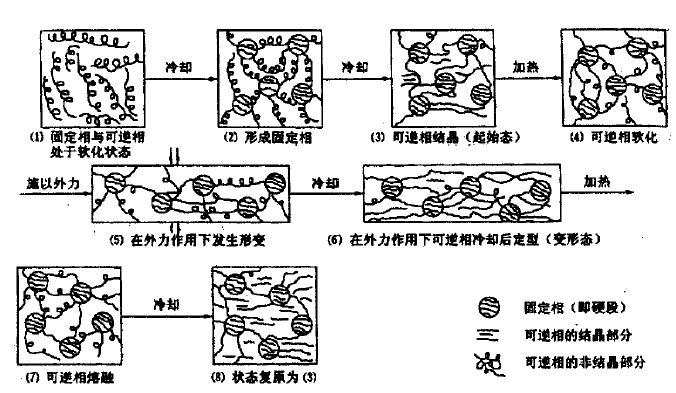
\includegraphics[width=0.75\textwidth]{figures/figure1}
 \caption{热塑性形状记忆聚氨酯的形状记忆机理示意图}\label{fig:diagram}
\end{figure}


\subsection{形状记忆聚氨酯的研究进展}
%\label{sec:requirements}
首例SMPU是日本Mitsubishi公司开发成功的……。

\subsection{水系聚氨酯及聚氨酯整理剂}

水系聚氨酯的形态对其流动性,成膜性及加工织物的性能有重要影响,一般分为三种类型\upcite{Jiang2005Size} ,如表 \ref{tab:category}所示。

\begin{table}
  \centering
  \caption{水系聚氨酯分类} \label{tab:category}
  \begin{tabular*}{0.9\textwidth}{@{\extracolsep{\fill}}cccc}
  \toprule
    类别			&水溶型		&胶体分散型		&乳液型 \\
  \midrule
    状态			&溶解$\sim$胶束	&分散		&白浊 \\
    外观			&水溶型		&胶体分散型		&乳液型 \\
    粒径$/\mu m$	&$<0.001$		&$0.001-0.1$		&$>0.1$ \\
    重均分子量	&$1000\sim 10000$	&数千$\sim 20万$ &$>5000$ \\
  \bottomrule
  \end{tabular*}
\end{table}

由于它们对纤维织物的浸透性和亲和性不同,因此在纺织品染整加工中的用途也有差别,其中以水溶型和乳液型产品较为常用。另外,水系聚氨酯又有反应性和非反应性之分。虽然它们的共同特点是分子结构中不含异氰酸酯基,但前者是用封闭剂将异氰酸酯基暂时封闭,在纺织品整理时复出。相互交联反应形成三维网状结构而固着在织物表面。
……

